\documentclass{beamer}
\usetheme{metropolis}
\usepackage{graphicx}
\usepackage{tcolorbox}
\usepackage{amsmath}
\usepackage{hyperref}
\usepackage{verbatim}
\DeclareMathOperator\erfc{erfc}
\DeclareMathOperator\Ei{Ei}
\definecolor{box_background}{RGB}{240,240,240}
\definecolor{box_frame}{RGB}{40,40,40}
\title{Complex analysis of Askaryan radiation: energy and angular reconstruction of ultra-high energy neutrinos}
\author{Jordan C. Hanson and Raymond Hartig}
\institute{Dept. of Physics and Astronomy \\ Whittier College \\ Whittier, CA}

\begin{document}
\titlegraphic{\vspace{6cm}\hspace{6.8cm}
\includegraphics[width=4cm,height=2cm]{WhittierImages.pdf}}  
\maketitle

\begin{frame}{Outline: from mathematical physics to UHE-$\nu$ observations}
\begin{columns}[T]
\begin{column}{0.5\textwidth}
\textbf{\alert{Background}}
\begin{itemize}
\item UHE-$\nu$ flux
\item The Askaryan effect
\item RF UHE-$\nu$ detectors
\end{itemize}
\textbf{\alert{The Askaryan signal}}
\begin{itemize}
\item Analytic radiation model
\item Signal \textit{envelopes}
\item Uncertainty principles
\end{itemize}
\textbf{\alert{Event reconstruction}}
\begin{itemize}
\item Mathematics $\leftrightarrow$ signals
\item \textbf{NuRadioMC}: MC software
\item Initial results
\end{itemize}
\end{column}
\begin{column}{0.5\textwidth}
\begin{figure}
\centering
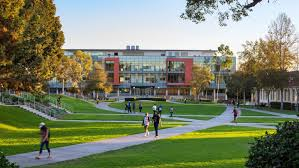
\includegraphics[width=0.9\textwidth]{whittier3.jpeg}
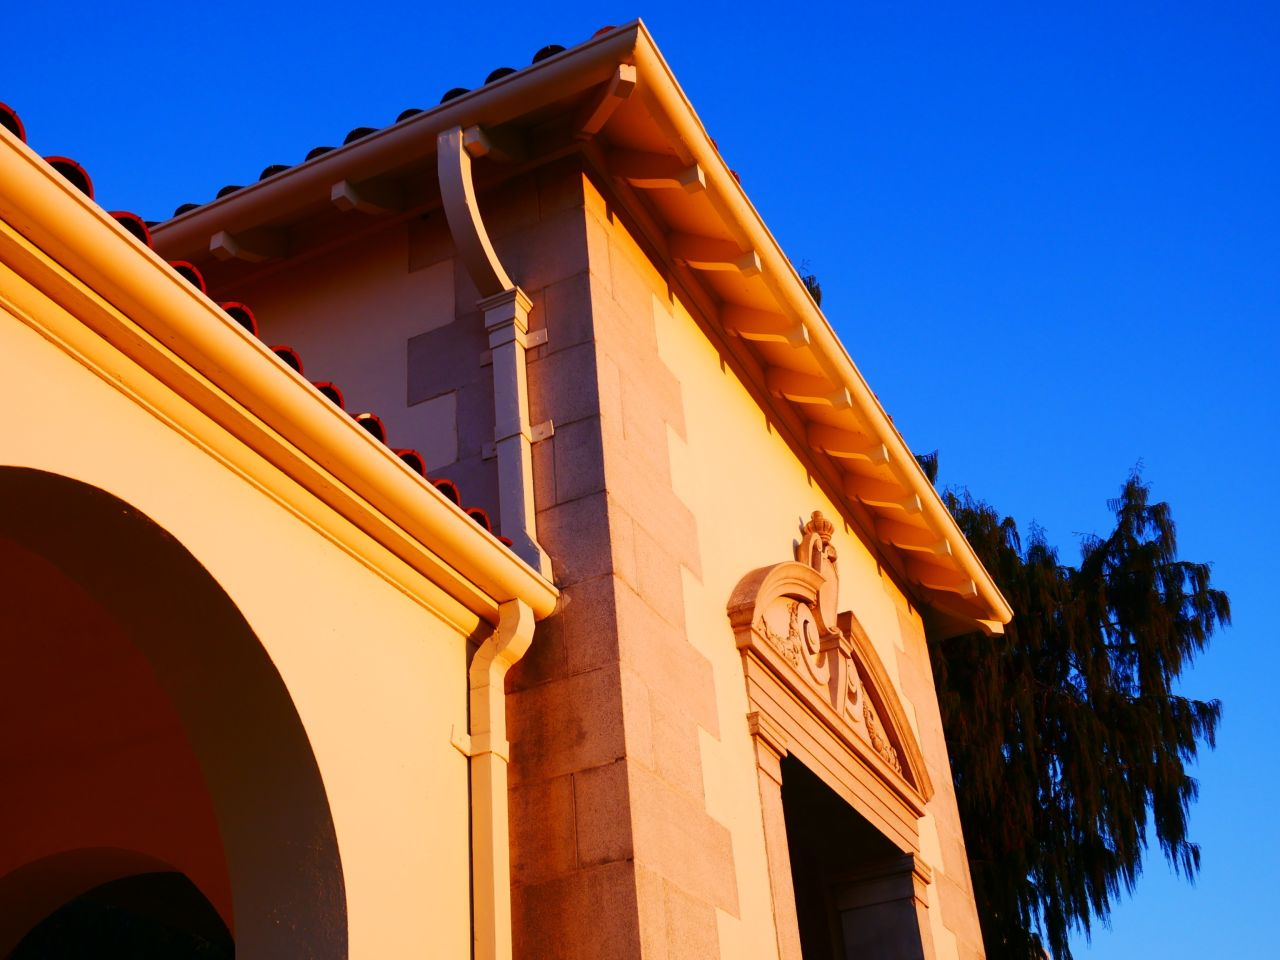
\includegraphics[width=0.9\textwidth]{whittier1.jpeg}
\caption{\small Whittier College.}
\end{figure}
\end{column}
\end{columns}
\end{frame}

\section{Background}

\begin{frame}{Background: in-ice UHE-$\nu$ observations}
\small
\begin{columns}[T]
\begin{column}{0.32\textwidth}
\textbf{\alert{UHE-$\nu$ detection via the Askaryan Effect}}
\begin{itemize}
\item \textbf{E$_{\nu} \geq $10$^{16}$ eV}
\item \textbf{Flux is small}
\item Cascades $\leftrightarrow$ RF
\item Ice is transparent
\item Station arrays
\end{itemize}
\end{column}
\begin{column}{0.68\textwidth}
\begin{figure}
\centering
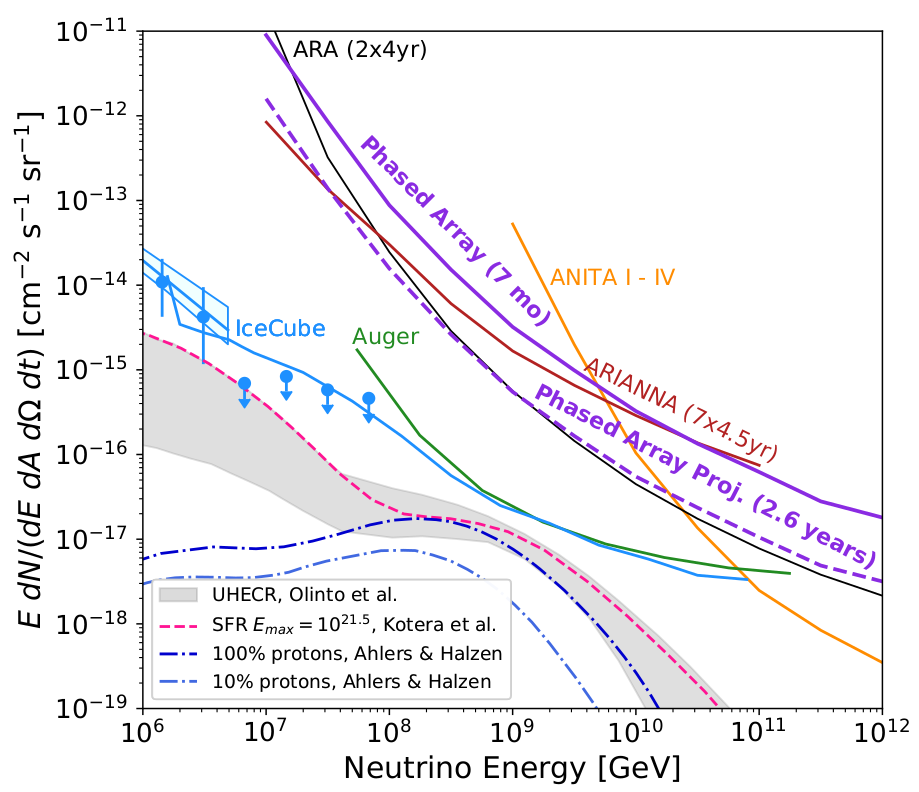
\includegraphics[width=0.9\textwidth]{flux.png}
\caption{\footnotesize UHE-$\nu$ flux predictions and upper limits.}
\end{figure}
\end{column}
\end{columns}
\end{frame}

\begin{frame}{Background: in-ice UHE-$\nu$ observations}
\small
\begin{columns}[T]
\begin{column}{0.32\textwidth}
\textbf{\alert{UHE-$\nu$ detection via the Askaryan Effect}}
\begin{itemize}
\item $E_{\nu} \geq 10^{16}$ eV
\item Flux is small
\item \textbf{Cascades $\leftrightarrow$ RF}
\item \textbf{Ice is transparent}
\item Station arrays
\end{itemize}
\end{column}
\begin{column}{0.68\textwidth}
\begin{figure}
\centering
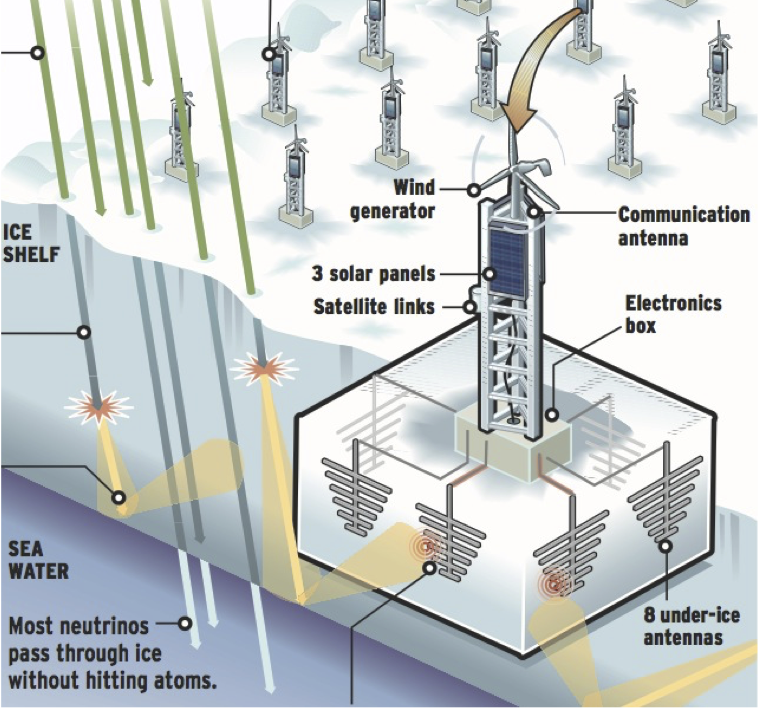
\includegraphics[width=0.45\textwidth]{ARIANNA_principle.png} \\
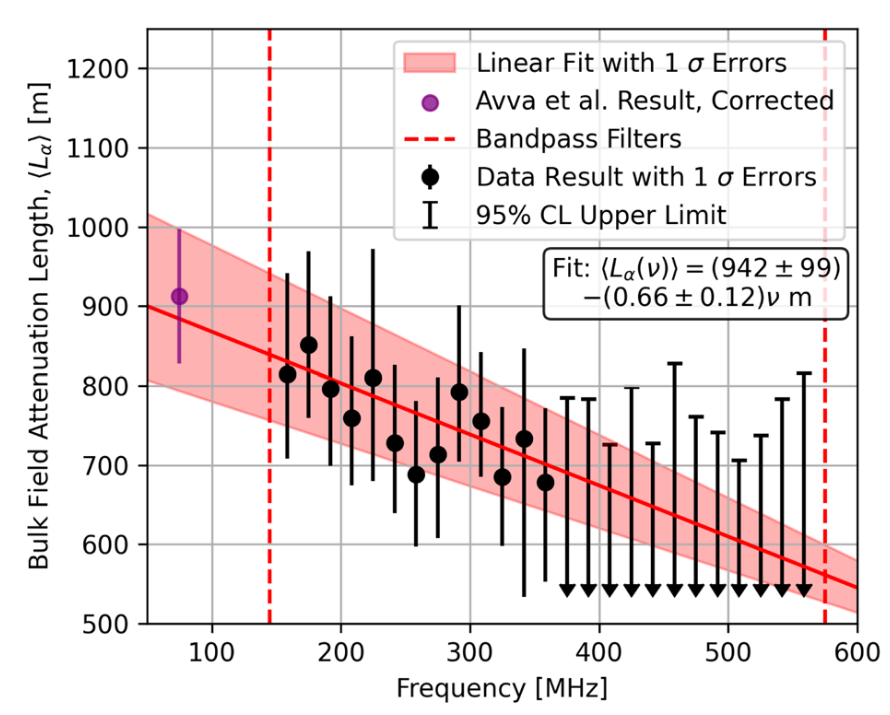
\includegraphics[width=0.55\textwidth]{atten_greenland.png}
\caption{\footnotesize (Top) Detectors use the Askaryan effect. (Bottom) RF attenuation lengths in ice.}
\end{figure}
\end{column}
\end{columns}
\end{frame}

\begin{frame}{Background: in-ice UHE-$\nu$ observations}
\small
\begin{columns}[T]
\begin{column}{0.32\textwidth}
\textbf{\alert{UHE-$\nu$ detection via the Askaryan Effect}}
\begin{itemize}
\item $E_{\nu} \geq 10^{16}$ eV
\item Flux is small
\item Cascades $\leftrightarrow$ RF
\item Ice is transparent
\item \textbf{Station arrays}
\end{itemize}
\end{column}
\begin{column}{0.68\textwidth}
\begin{figure}
\centering
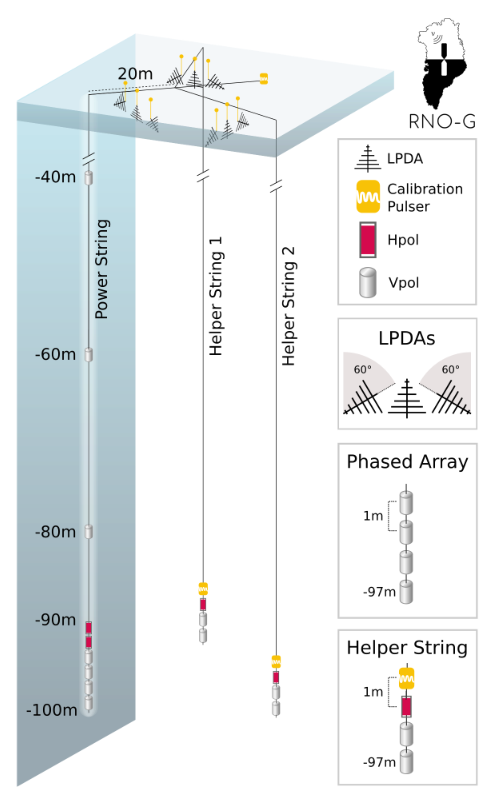
\includegraphics[width=0.35\textwidth]{RNO-G.png} \hspace{0.5cm}
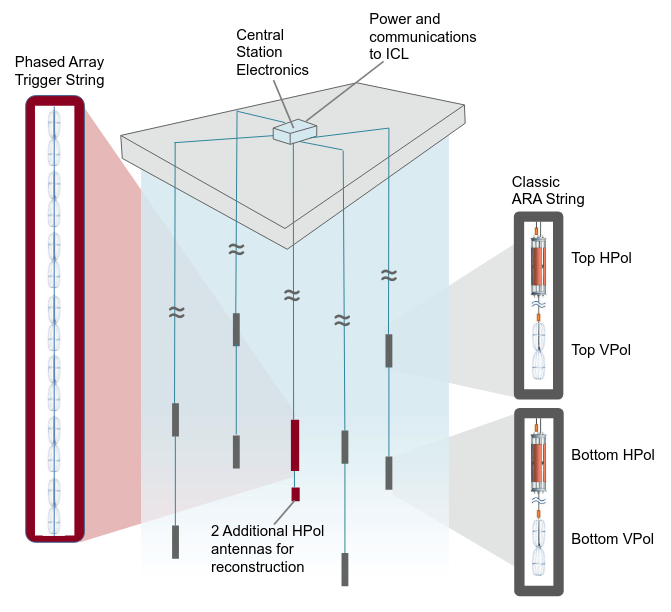
\includegraphics[width=0.55\textwidth]{ARA.png}
\caption{\footnotesize In-ice UHE-$\nu$ detectors. (Left) RNO-G (Greenland). (Right) ARA (Antarctica).}
\end{figure}
\end{column}
\end{columns}
\end{frame}

\section{The Askaryan Signal}

\begin{frame}{The Askaryan Signal: equation for $\vec{E}$-field}
\begin{tcolorbox}[colback=box_background,colframe=box_frame,title={Askaryan electric field, $\vec{E}(r,t)$, [V m$^{-1}$]}]
\begin{equation}
r \vec{E}(t,\theta) = -\frac{E_0 \omega_0 \sin(\theta)}{8 \pi p} t_r e^{-\frac{t_r^2}{4p} + p \omega_0^2}\erfc(\sqrt{p}\omega_0)
\end{equation}
\end{tcolorbox}
\footnotesize
\begin{columns}[T]
\begin{column}{0.49\textwidth}
\textbf{Geometric parameters}
\begin{table}
\centering
\begin{tabular}{c|c}
$r$ & vertex distance [m] \\
$E_0$ & E-field amplitude [V GHz$^{-2}$] \\
$t_r$ & Retarded time [ns]\footnote{Definition: $t_{\rm r} = t_{\rm ref} - nR/c$.} \\
$\theta$ & Observation angle [rad] \\
$p$ & $\sigma_t = \sqrt{2p}$ (Eq. \ref{eq:p}) [ns$^2$]
\end{tabular}
\end{table}
\end{column}
\begin{column}{0.49\textwidth}
\textbf{Particle physics parameters}
\begin{table}
\centering
\begin{tabular}{c|c}
$\omega_0$ & Form-factor frequency [GHz] \\
$\theta_{\rm C}$ & Cherenkov angle [rad] \\
$p$ & $\sigma_t = \sqrt{2p}$ (Eq. \ref{eq:p}) [ns$^2$] \\
$a$ & Cascade length (Eq. \ref{eq:p}) [m]
\end{tabular}
\end{table}
\begin{align}
p =& \frac{1}{2}\left(\frac{a}{c}\right)^2 \left(\cos\theta - \cos\theta_C\right)^2 \label{eq:p} \\
\sqrt{2p} \approx & ~(a/c)|\theta - \theta_{\rm C}|\sin\theta_{\rm C} \\
\sigma_t =& \sqrt{2p} \propto ~ a\Delta\theta
\end{align}
\end{column}
\end{columns}
\end{frame}

\begin{frame}{The Askaryan Signal: $\vec{E}$-field time-dependence, analytic signal}
\begin{tcolorbox}[colback=box_background,colframe=box_frame,title={Askaryan electric field, $\vec{E}(r,t)$, [V m$^{-1}$], time-dependence}]
\begin{equation}
s(t) = \vec{E}(t,\theta) = -E_0 t e^{-\frac{1}{2}\left(\frac{t}{\sigma_t}\right)^2}
\end{equation}
\end{tcolorbox}
\begin{tcolorbox}[colback=box_background,colframe=box_frame,title={Askaryan electric field \textit{analytic signal}}]
\begin{equation}
s_a(t) = -E_0 \left(t e^{-\frac{1}{2}\left(t/\sigma_t\right)^2} - \frac{2 j\sigma_t}{\sqrt{2\pi}} \frac{dD(x)}{dx}\right)
\end{equation}
\end{tcolorbox}
\footnotesize
\begin{columns}[T]
\begin{column}{0.49\textwidth}
\textbf{The signal envelope}
\begin{itemize}
\item $s_a(t) = s(t) + j ~ \widehat{s}(t)$
\item $\widehat{s}(t)$, Hilbert transform
\item $|s_a(t)|$, signal \textit{envelope}
\end{itemize}
\end{column}
\begin{column}{0.49\textwidth}
\textbf{Special functions and variables}
\begin{itemize}
\item $D(x)$, Dawson function
\item $x = t/(\sqrt{2}\sigma_t)$, normalized time
\end{itemize}
\end{column}
\end{columns}
\end{frame}

\begin{frame}{The Askaryan Signal: detected signals}
\begin{tcolorbox}[colback=box_background,colframe=box_frame,title={Common response function for RF channels $r(t)$, [m ns$^{-1}$]}]
\begin{equation}
r(t) = R_0 \cos(2\pi f_0 t) e^{-\gamma t}
\end{equation}
\end{tcolorbox}
\begin{tcolorbox}[colback=box_background,colframe=box_frame,title={Common analytic signal for RF channels $r_a(t)$, [m ns$^{-1}$]}]
\begin{equation}
r_a(t) = R_0 e^{2\pi j f_0 t-\gamma t}
\end{equation}
\end{tcolorbox}
\footnotesize
\begin{columns}[T]
\begin{column}{0.49\textwidth}
\textbf{The signal envelope}
\begin{itemize}
\item $r_a(t) = r(t) + j ~ \widehat{r}(t)$
\item $\widehat{r}(t)$, Hilbert transform
\item $|r_a(t)|$, signal \textit{envelope}
\end{itemize}
\end{column}
\begin{column}{0.49\textwidth}
\textbf{RF channels: RLC circuits}
\begin{itemize}
\item $|r_a(t)| = R_0\exp(-\gamma t)$
\item $\gamma$, damping coefficient [GHz]
\item $f_0$, resonance frequency [GHz]
\end{itemize}
\end{column}
\end{columns}
\end{frame}

\begin{frame}{The Askaryan Signal: detected signals}
\begin{tcolorbox}[colback=box_background,colframe=box_frame,title={Detected signals, $r(t) * s(t)$, [V]}]
\begin{equation}
r(t) * s(t) = \int_{-\infty}^{\infty} r(\tau) s(t-\tau) d\tau \rightarrow \int_{0}^{\infty} r(\tau) s(t-\tau) d\tau
\end{equation}
\end{tcolorbox}
\begin{tcolorbox}[colback=box_background,colframe=box_frame,title=Theorem: the envelope of detected signal]
Let $\mathcal{E}_{r * s}(t)$ represent the \textit{envelope} of the convolution of $r(t)$ and $s(t)$.  If $s_a(t)$ and $r_a(t)$ are the analytic signals of $s(t)$ and $r(t)$, respectively, then
\begin{equation}
\mathcal{E}_{r*s}(t) = \frac{1}{2}|r_a(t) * s_a(t)|
\end{equation}
\end{tcolorbox}
\end{frame}

\begin{frame}{The Askaryan Signal: uncertainty principles}
\begin{tcolorbox}[colback=box_background,colframe=box_frame,title={Uncertainty principles within Askaryan field}]
Let $\Delta\theta = \theta - \theta_{\rm C}$.  Let $a$ be the cascade length, $c$ be the speed of light, $\sigma_t$ be the pulse width, and $\sigma_f$ be the width of the Fourier spectrum.
\begin{equation}
a\Delta\theta = \frac{c\sigma_t}{\sin\theta_{\rm C}}
\end{equation}
Further, $s(t)$, and $S(f)$ (the Fourier transform), have widths that satisfy
\begin{equation}
\sigma_t \sigma_f = \frac{1}{2\pi}\left(1+\eta^2\right)^{1/2}
\end{equation}
In the far-field, $\eta \to 0$.
\end{tcolorbox}
\end{frame}

\begin{frame}[fragile]{The Askaryan Signal: scanning $a$ and $\Delta\theta$}
\begin{figure}
\centering
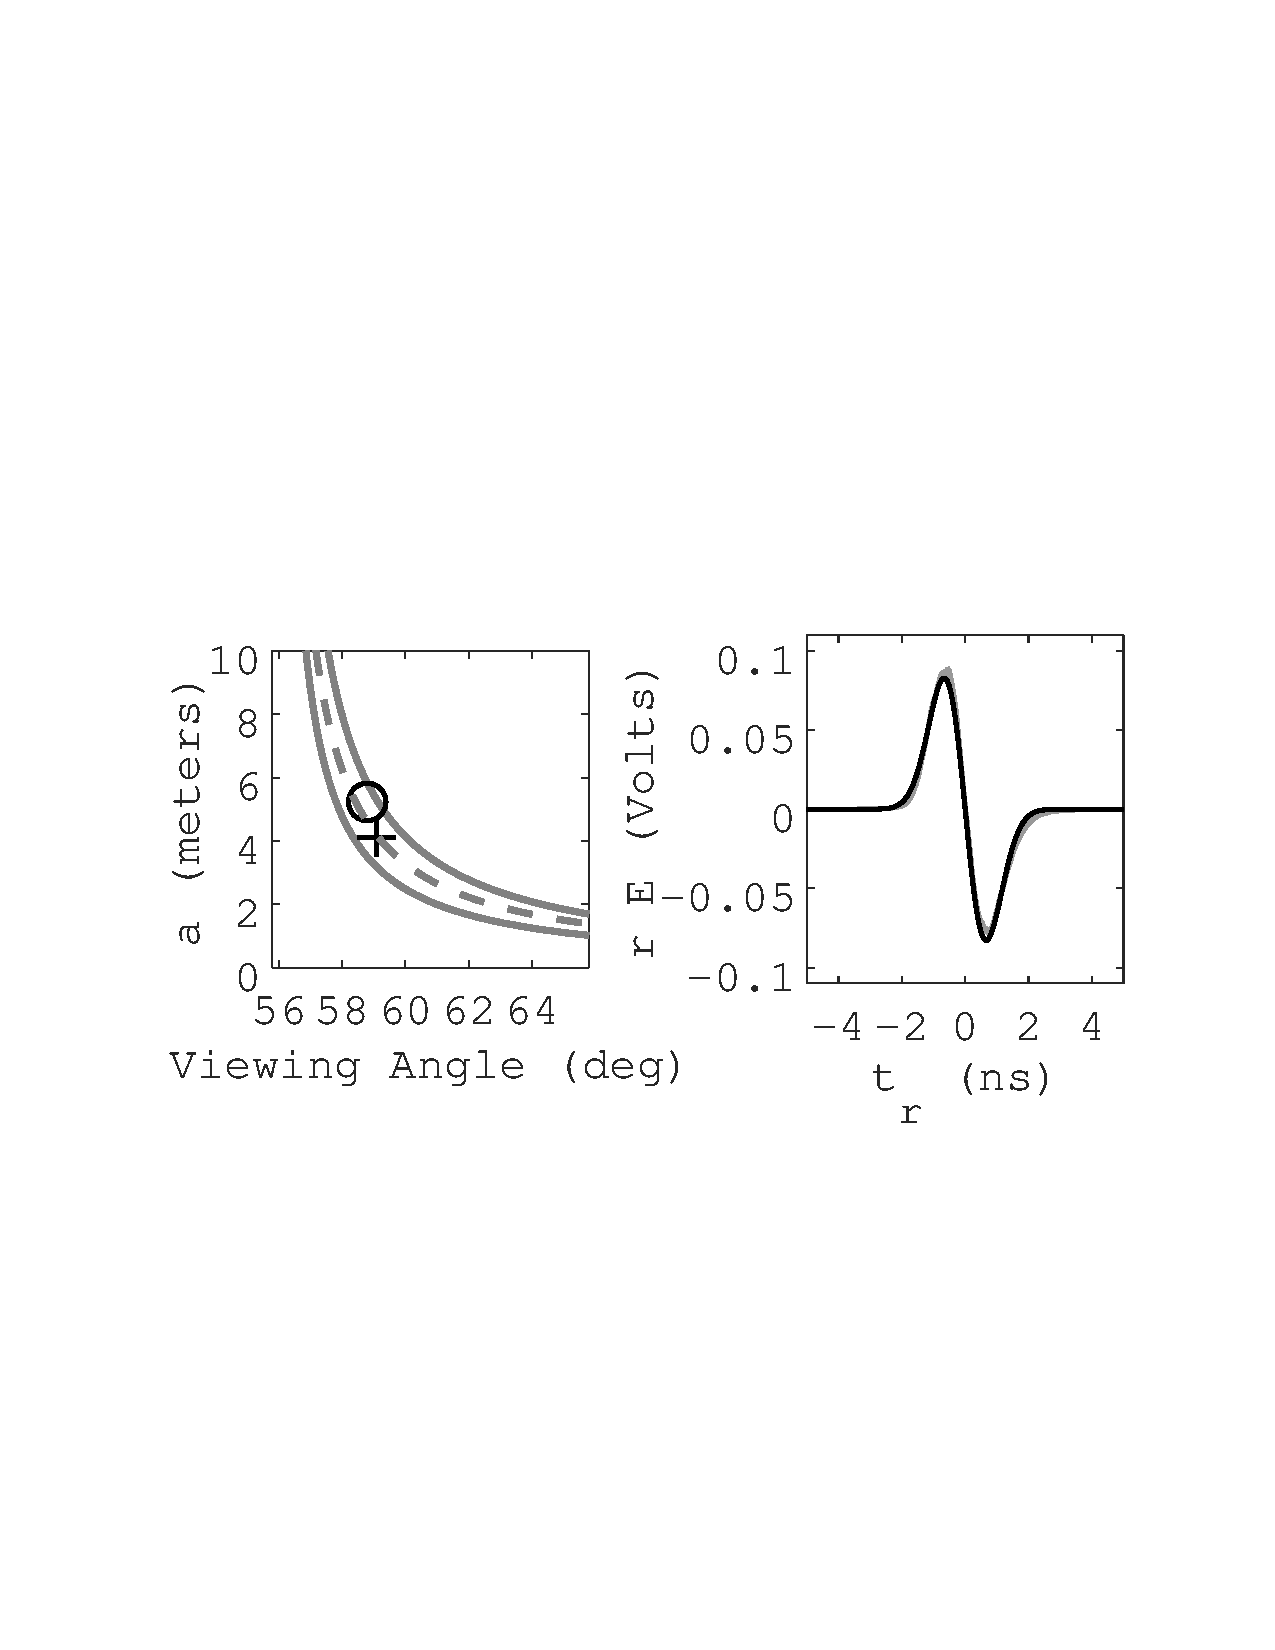
\includegraphics[width=0.9\textwidth,trim=2cm 9cm 2cm 10cm,clip=true]{example_scan.pdf}
\caption{\footnotesize \label{fig:scan} Fitting Askaryan field to NuRadioMC output. (Left) reconstruction of $a$ and $\Delta\theta$, mathematical $\vec{E}$-field vs. MC $\vec{E}$-field.  Circle: MC true.  Cross: reconstruction.}
\end{figure}
\textbf{Energy reconstruction potential:} $a^2 \propto \ln(E_{\rm C}/E_{\rm crit})$
\end{frame}

\section{Event Reconstruction}

\begin{frame}[fragile]{Event Reconstruction: calculating $\mathcal{E}_{r * s}(t)$}
\textbf{\alert{Stages of the calculation:}}
\begin{itemize}
\item Calculate $r_a(t)$ and $s_a(t)$ (already shown).
\item Convolve $r_a(t)$ and $\Re\lbrace s_a(t)\rbrace$ (time domain).
\item Convolve $r_a(t)$ and $\Im\lbrace s_a(t)\rbrace$ (Fourier domain).
\item Combine results and take the magnitude, multiply by $(1/2)$.
\end{itemize}
\end{frame}

\begin{frame}[fragile]{Event Reconstruction: $r_a(t) * \Re\lbrace s_a(t)\rbrace$}
\begin{tcolorbox}[colback=box_background,colframe=box_frame,title={Result for $r_a(t) * \Re\lbrace s_a(t)\rbrace$}]
\begin{multline}
r_a(t) * \Re\lbrace s_a(t) \rbrace = \sqrt{\frac{\pi}{2}}R_0 \sigma_t s(t) w(z) \\
+ R_0 E_0 \sigma_t^2 e^{-\frac{1}{2}(t/\sigma_t)^2}(1+j\sqrt{\pi} z w(z)) \label{eq:Re_result}
\end{multline}
\end{tcolorbox}
\small
\begin{columns}[T]
\begin{column}{0.49\textwidth}
\textbf{Complex poles:}
\begin{itemize}
\item $z_1 = f_0/(\sqrt{2}\sigma_f) + j\gamma/(2\pi \sqrt{2} \sigma_f)$
\item $z_1 = z + jx$
\end{itemize}
\end{column}
\begin{column}{0.49\textwidth}
\textbf{The Faddeeva function}
\begin{itemize}
\item $w(z) = e^{-z^2}\erfc(-jz)$
\item $w(z) = e^{y^2}\erfc(y)$, $z\to jy$
\end{itemize}
\end{column}
\end{columns} \vspace{0.25cm}
\normalsize
\textbf{\alert{Combine real and imaginary parts:}} $\mathcal{E}_{r * s}(t) = \frac{1}{2}|r_a(t) * s_a(t)|$
\end{frame}

\begin{frame}[fragile]{Event Reconstruction: $r_a(t) * \Im\lbrace s_a(t)\rbrace$}
\begin{tcolorbox}[colback=box_background,colframe=box_frame,title={Result for $r_a(t) * \Im\lbrace s_a(t)\rbrace$}]
\begin{multline}
r_a(t) * \Im\left\lbrace s_a(t) \right\rbrace = \\
\sqrt{\pi}E_0 \sigma_t^2 z_1 e^{-z_1^2}r_a(t) + \sqrt{\frac{2}{\pi}} G(z_1) R_0 \sigma_t s(t) \label{eq:Im_result}
\end{multline}
\end{tcolorbox}
\small
\begin{columns}[T]
\begin{column}{0.49\textwidth}
\textbf{Complex poles:}
\begin{itemize}
\item $z_1 = f_0/(\sqrt{2}\sigma_f) + j\gamma/(2\pi \sqrt{2} \sigma_f)$
\item $z_1 = z + jx$
\end{itemize}
\end{column}
\begin{column}{0.49\textwidth}
\textbf{The Goodwin-Staton integral}
\begin{itemize}
\item $G(z) = \sqrt{\pi}F(z) - \frac{1}{2}e^{-z^2}\Ei(z^2)$
\item $\Ei(z)$ is an exponential integral
\end{itemize}
\end{column}
\end{columns} \vspace{0.25cm}
\normalsize
\textbf{\alert{Combine real and imaginary parts:}} $\mathcal{E}_{r * s}(t) = \frac{1}{2}|r_a(t) * s_a(t)|$
\end{frame}

\begin{frame}[fragile]{Event Reconstruction: graphs of $\mathcal{E}_{r * s}(t)$}
\begin{figure}
\centering
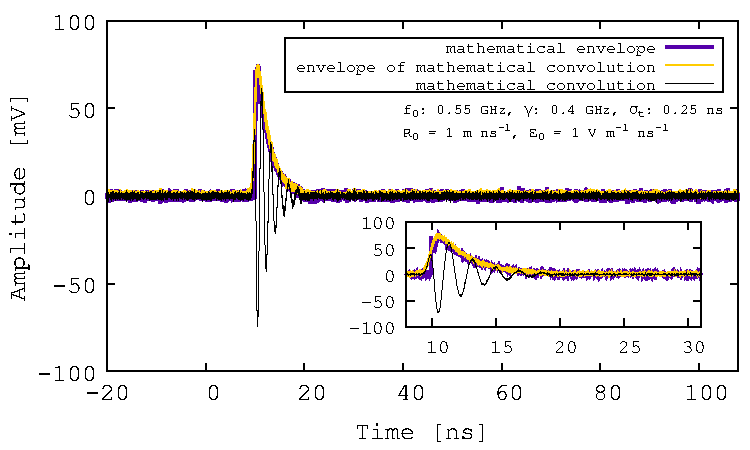
\includegraphics[width=\textwidth]{March12_plot1.pdf}
\caption{\footnotesize \label{fig:fig1} Black line: $s(t) * r(t)$.  Gold line: the envelope of $s(t) * r(t)$ computed with the Python3 package scipy.special.hilbert. Purple line: $\mathcal{E}_{r * s}(t)$.}
\end{figure}
\end{frame}

\begin{frame}[fragile]{Event Reconstruction: graphs of $\mathcal{E}_{r * s}(t)$}
\begin{figure}
\centering
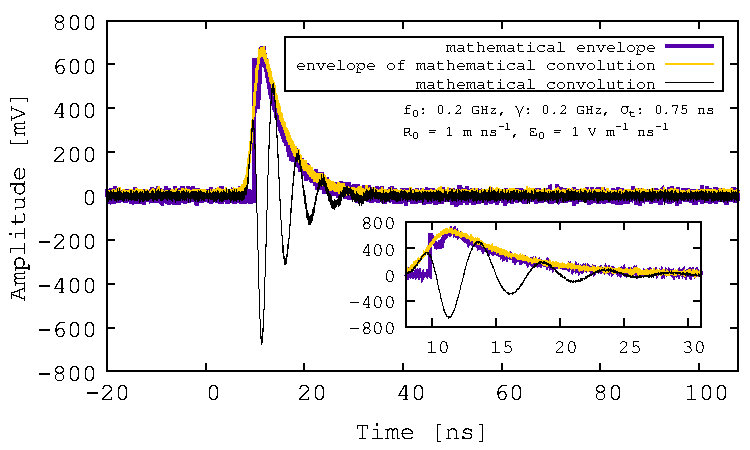
\includegraphics[width=\textwidth]{March12_plot2.pdf}
\caption{\footnotesize \label{fig:fig2} Same is Fig. \ref{fig:fig1}, with different parameters.}
\end{figure}
\end{frame}

\begin{frame}[fragile]{Event Reconstruction: (prelim.) reconstructed $a$ vs. $\Delta\theta$}
\begin{figure}
\centering
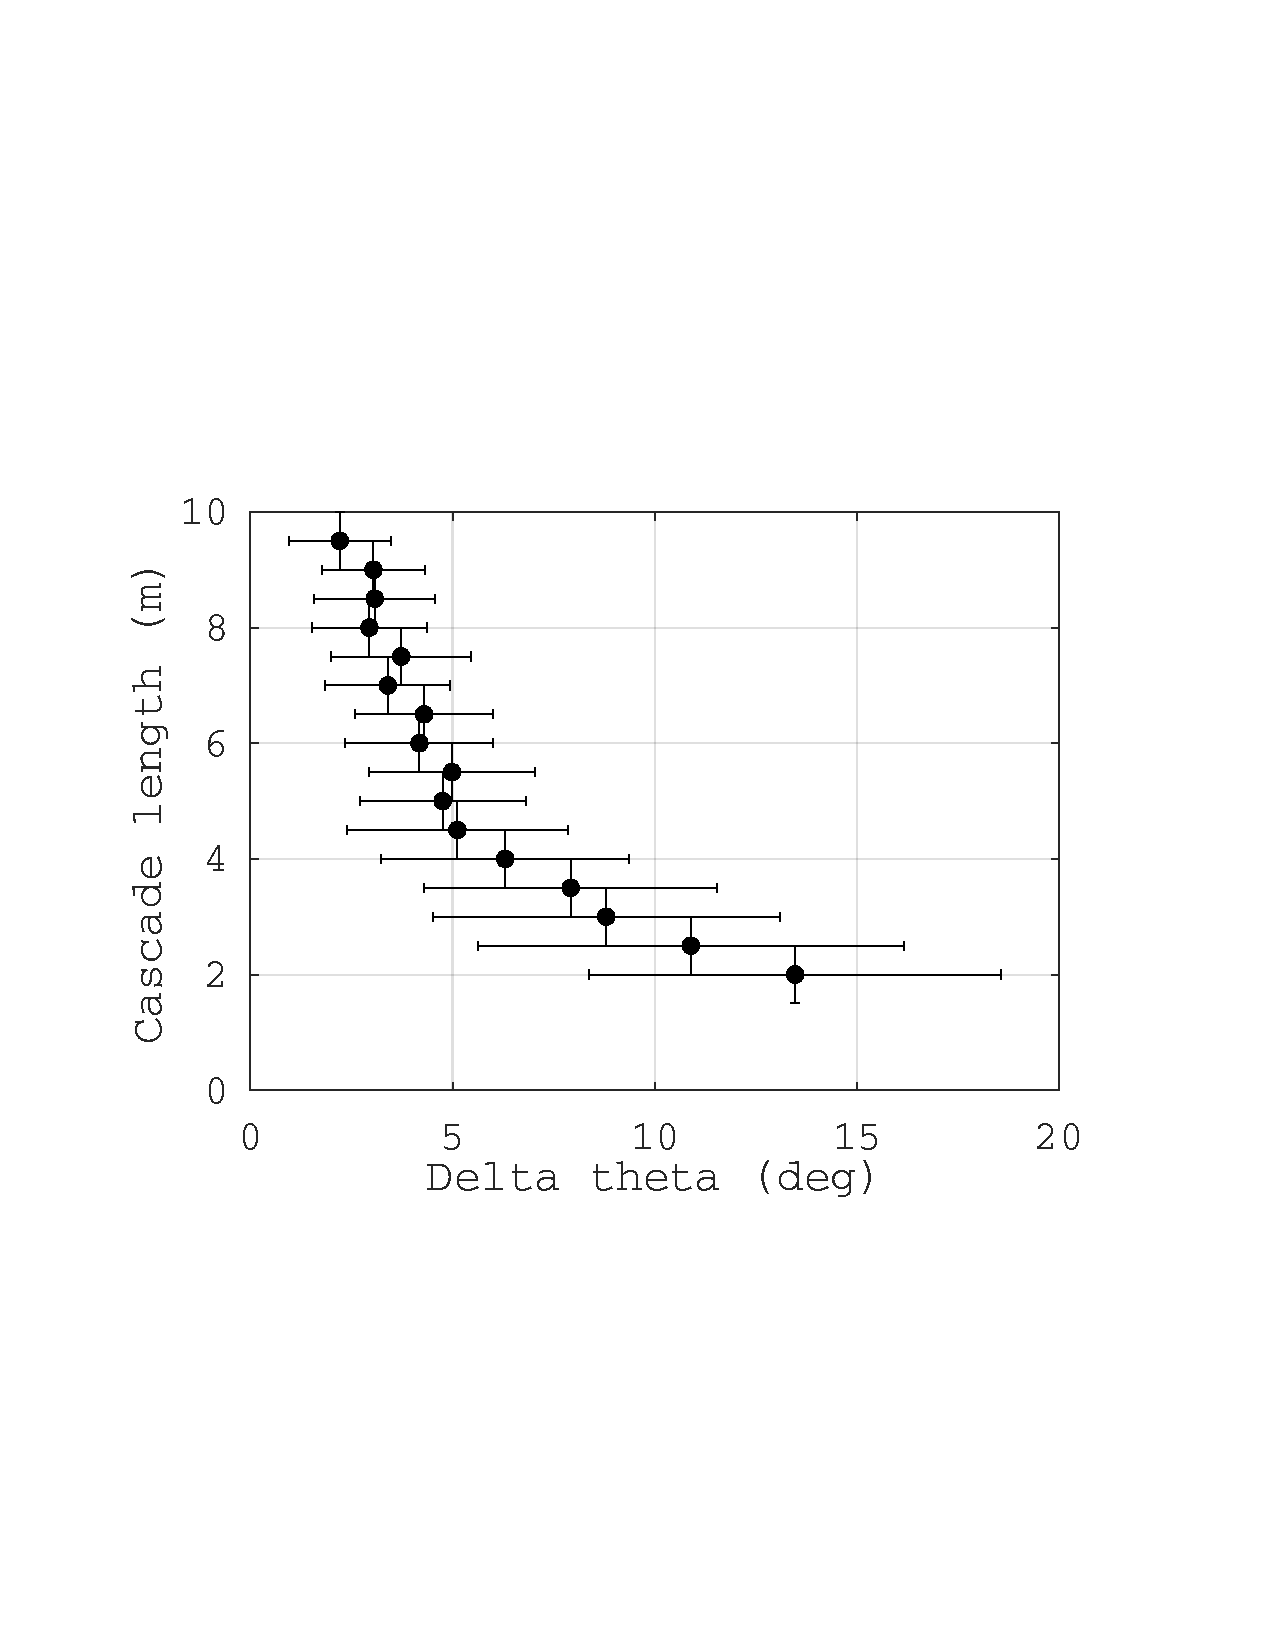
\includegraphics[width=0.55\textwidth,height=0.5\textwidth,trim=0cm 7cm 3cmcm 5cm,clip=true]{March14_plot1.pdf}
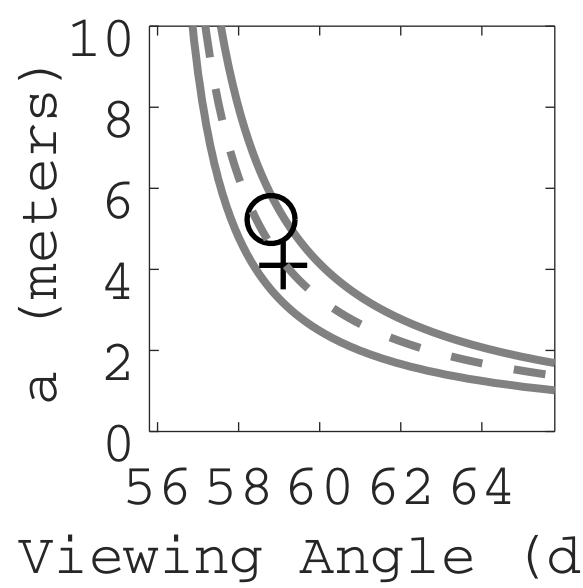
\includegraphics[width=0.4\textwidth]{scan_grab.png}
\caption{\footnotesize \label{fig:fig3} (Left) Reconstructed $a$ and $\Delta\theta$, from NuRadioMC. (Right) Fig. \ref{fig:scan} (right), for comparison.}
\end{figure}
\end{frame}

\section{Conclusion}

\begin{frame}{Outline: from mathematical physics to UHE-$\nu$ observations}
\begin{columns}[T]
\begin{column}{0.5\textwidth}
\textbf{\alert{Background}}
\begin{itemize}
\item UHE-$\nu$ flux
\item The Askaryan effect
\item RF UHE-$\nu$ detectors
\end{itemize}
\textbf{\alert{The Askaryan signal}}
\begin{itemize}
\item Analytic radiation model
\item Signal \textit{envelopes}
\item Uncertainty principles
\end{itemize}
\textbf{\alert{Event reconstruction}}
\begin{itemize}
\item Mathematics $\leftrightarrow$ signals
\item \textbf{NuRadioMC}: MC software
\item Initial results
\end{itemize}
\end{column}
\begin{column}{0.5\textwidth}
\begin{figure}
\centering
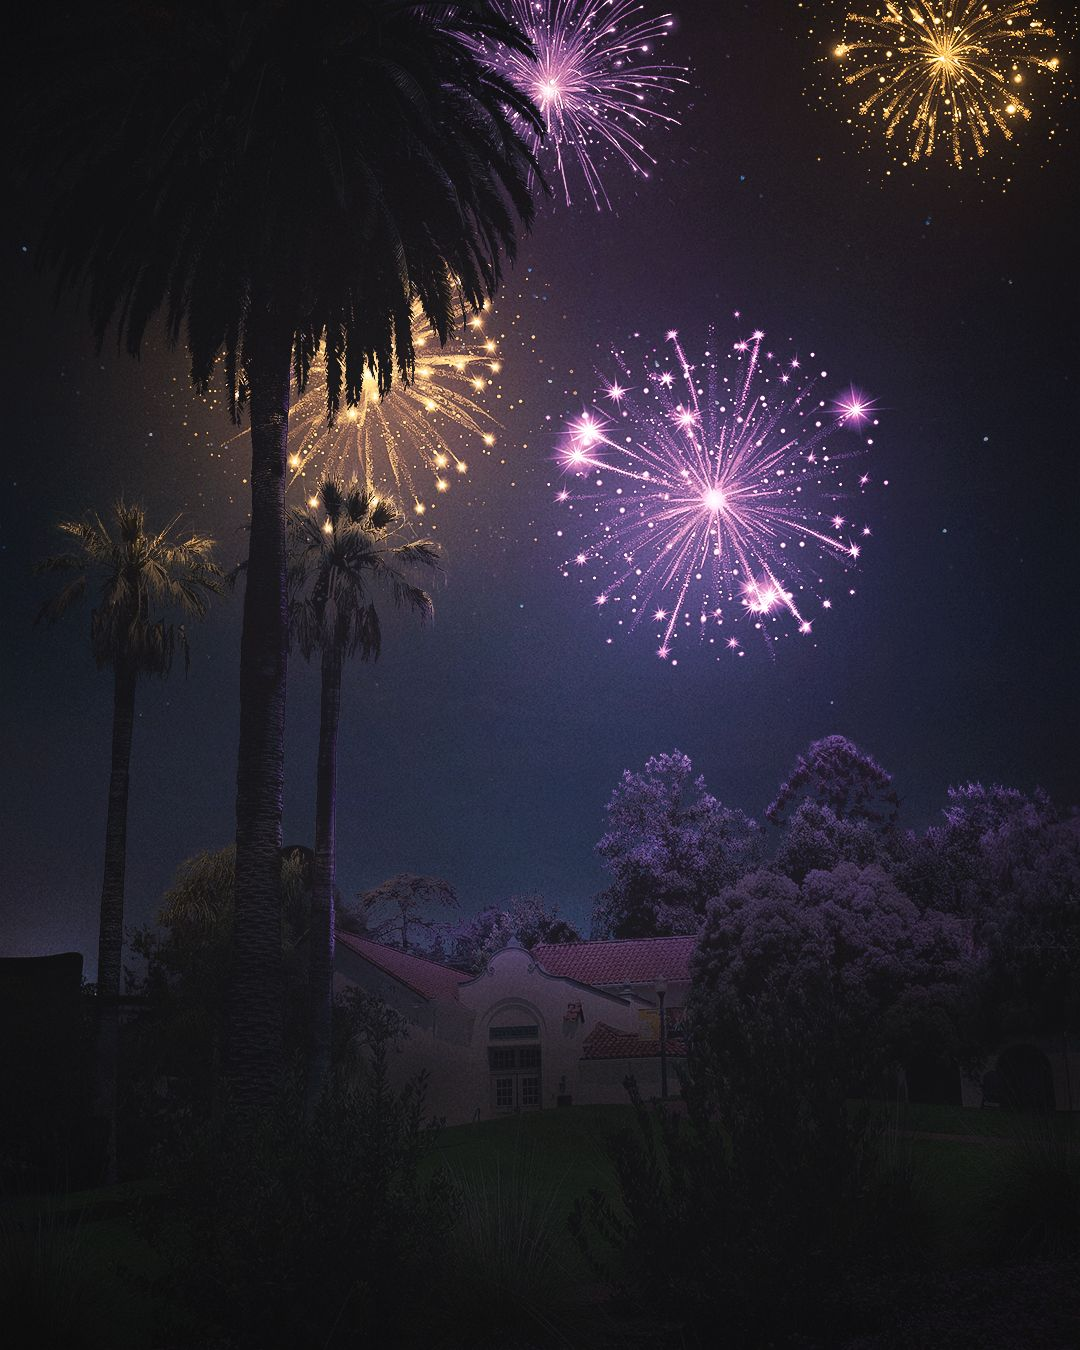
\includegraphics[width=0.9\textwidth]{whittier2.jpeg}
\caption{\small Whittier College.}
\end{figure}
\end{column}
\end{columns}
\end{frame}

\section{References}

\begin{frame}{References}
\footnotesize
\begin{enumerate}
\item P. Allison et al., Low-threshold ultrahigh-energy neutrino search with the Askaryan Radio Array, Phys Rev D 105, 122006 (2022).
\item J. A. Aguilar et al., In situ, broadband measurement of the radio frequency attenuation length at Summit Station, Greenland, J. Glaciol. 68, 1234 (2022).
\item S. Agarwal et al., Instrument design and performance of the first seven stations of RNO-G, arXiv (2024).
\item \textbf{J. C. Hanson and R. Hartig}, Complex analysis of Askaryan radiation: A fully analytic model in the time domain, Phys Rev D 105, 123019 (2022).
\item \textbf{J. C. Hanson and A. L. Connolly}, Complex analysis of Askaryan radiation: A fully analytic treatment including the LPM effect and Cascade Form Factor, Astroparticle Physics 91, 75 (2017).
\item C. Glaser et al., NuRadioMC: simulating the radio emission of neutrinos from interaction to detector, European Phys J C 80, 77 (2020).
\end{enumerate}
\end{frame}

\section{Bonus Slides}

\begin{frame}[fragile]{Calculate the signal envelope with SciPy}
\begin{verbatim}
import numpy as np
import scipy.signal.hilbert as hilbert
env_out = np.abs(hilbert(sig_in))
\end{verbatim}
\begin{enumerate}
\item The hilbert function computes the \textit{analytic signal}
\item The absolute value of the analytic signal is the envelope
\end{enumerate}
\end{frame}

\begin{frame}[fragile]{Calculate the envelope of the convolution of two functions}
\small
\begin{verbatim}
import numpy as np
import scipy.signal.hilbert as hilbert
env_out = 0.5*np.abs(np.conv(
    hilbert(sig_in_1),
    hilbert(sig_in_2),
    'same'))
\end{verbatim}
This is equivalent to:
\begin{verbatim}
import numpy as np
import scipy.signal.hilbert as hilbert
env_out = np.abs(hilbert(
    np.conv(sig_in_1,sig_in_2,'same')))
\end{verbatim}
\end{frame}

\end{document}
